
\section{Wyniki eksperymentów}
\label{sec:wyniki}

Do oceny wydajności i zachowania modelu wybrano eksperyment z najlepszymi artefaktami kodowymi, którego logi i dane wykresów zostały wyeksportowane do katalogu \texttt{best\_results/}. Analiza opiera się na przebiegu treningu trwającym ponad \num{22800} kroków.

W tabeli~\ref{tab:metryki-comet} przedstawiono wybrane końcowe metryki walidacyjne zarejestrowane w platformie Comet ML dla kroku \num{40299}. Dla dokładniejszego zbadania zachowania modelu w czasie treningu przeanalizowano dodatkowe charakterystyki opisane poniżej.

\input{tables/comet_metrics}

\subsection{Zachowanie straty przy różnych poziomach szumu}

Model dyfuzyjny w trakcie treningu uczy się rekonstrukcji tokenów przy różnym natężeniu szumu (różnych proporcjach maskowania kodu). Rysunek~\ref{fig:val-loss-masking} przedstawia przebieg straty walidacyjnej (\textit{Validation Loss}) dla czterech dyskretnych poziomów maskowania: \num{25}\%, \num{50}\%, \num{75}\% oraz \num{95}\%, a także ogólną średnią stratę walidacyjną.

\begin{figure}[htbp]
\centering
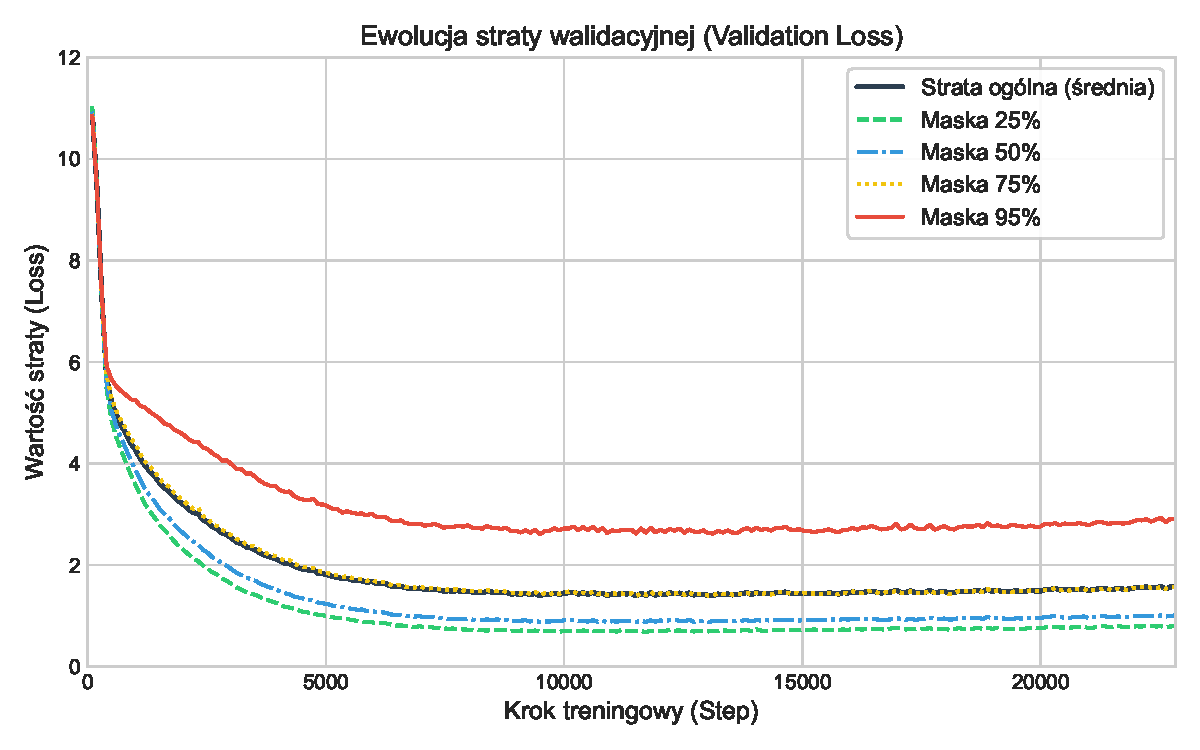
\includegraphics[width=0.85\linewidth]{figures/val_loss_masking}
\caption{Przebieg straty walidacyjnej w zależności od stopnia zamaskowania kodu (proporcji szumu) w trakcie treningu.}
\label{fig:val-loss-masking}
\end{figure}

Z wykresu wynika, że strata dla maskowania \num{25}\% (\textit{zielona linia przerywana}) jest najniższa i spada najszybciej, osiągając wartość końcową ok. \num{0.68}. Jest to zgodne z intuicją, ponieważ model, mając dostęp do \num{75}\% oryginalnego kodu (wysoki kontekst), ma znacznie ułatwione zadanie rekonstrukcji pozostałych tokenów. Z kolei strata dla maskowania \num{95}\% (\textit{czerwona linia ciągła}) reprezentuje sytuację ekstremalną, w której model musi zrekonstruować niemal cały kod wyłącznie na podstawie instrukcji naturalnojęzykowej i nielicznych tokenów pomocniczych. Ta strata również wykazuje tendencję spadkową w trakcie treningu (z poziomu ok. \num{10.8} do ok. \num{2.6}), co dowodzi, że model uczy się generowania kodu od podstaw. Wszystkie krzywe charakteryzują się gładką zbieżnością bez wyraźnych oznak przeuczenia (overfittingu) w badanym zakresie kroków, co potwierdza stabilność procesu treningowego.

\subsection{Wrażliwość modelu na instrukcje (Prompt Shuffling)}

Kluczową cechą warunkowego modelu generowania kodu jest jego sterowalność za pomocą instrukcji w języku naturalnym (promptu). Aby sprawdzić, czy model rzeczywiście bierze pod uwagę treść instrukcji, czy jedynie uczy się bezwarunkowego rozkładu kodu, zastosowano procedurę zaburzania kontekstu (\textit{Prompt Shuffling}). Polega ona na losowym przetasowaniu tokenów promptu podczas walidacji przy pełnym zamaskowaniu kodu (\num{100}\%).

Rysunek~\ref{fig:val-prompt-shuffle} przedstawia porównanie straty walidacyjnej przy oryginalnym promptcie (\textit{Original Prompt}) oraz przy zaburzonym promptcie (\textit{Shuffled Prompt}), a także różnicę między nimi (\textit{Delta}).

\begin{figure}[htbp]
\centering
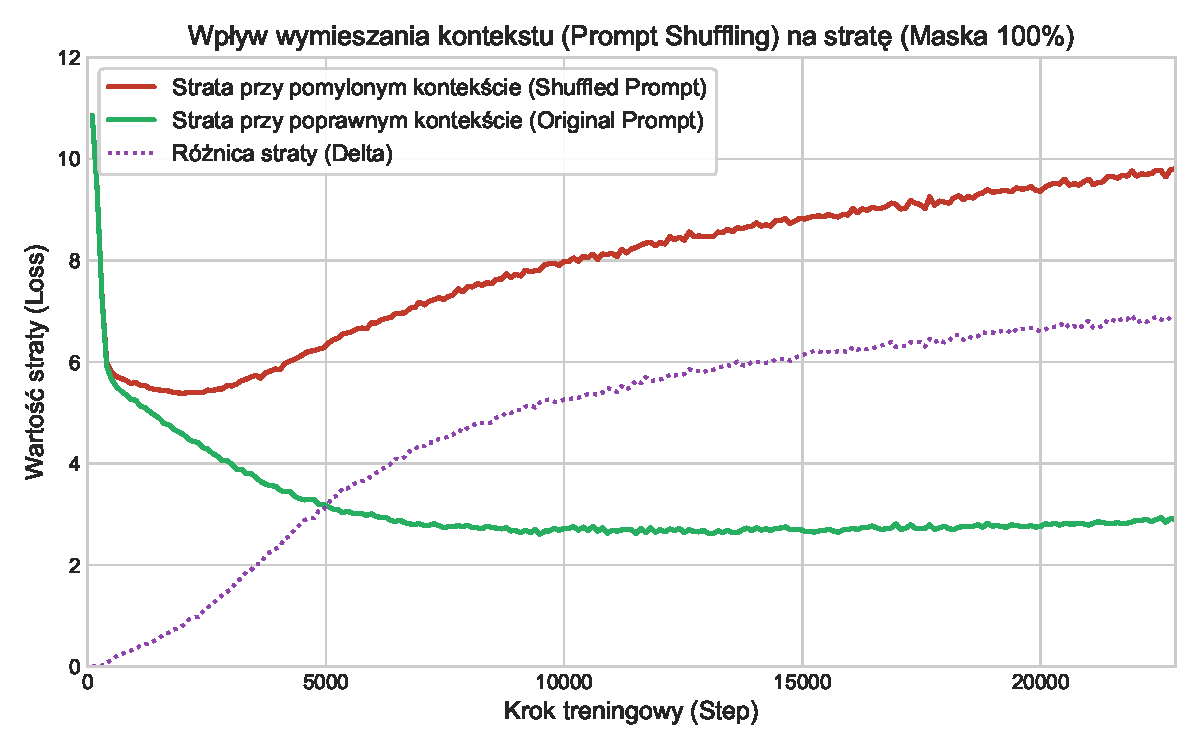
\includegraphics[width=0.85\linewidth]{figures/val_prompt_shuffle}
\caption{Wpływ przetasowania tokenów instrukcji (Prompt Shuffling) na wartość straty walidacyjnej przy maskowaniu \num{100}\%.}
\label{fig:val-prompt-shuffle}
\end{figure}

Analiza wykresu wskazuje na wyraźne różnice w zachowaniu modelu w zależności od poprawności instrukcji warunkującej. Strata przy zaburzonym promptcie (\textit{czerwona linia}) pozostaje na bardzo wysokim poziomie w trakcie całego treningu, spadając jedynie nieznacznie z ok. \num{10.8} do ok. \num{5.4}. W tym samym czasie strata przy poprawnym promptcie (\textit{zielona linia}) zbiega do wartości ok. \num{1.4}. W konsekwencji różnica straty (\textit{fioletowa linia przerywana}) rośnie w miarę postępu treningu, osiągając ostatecznie wartość ok. \num{6.9}. Wynik ten jednoznacznie potwierdza, że model rozwija silną zależność od struktury i semantyki promptu. Gdy instrukcja jest pozbawiona sensu wskutek przetasowania tokenów, zdolność modelu do poprawnej rekonstrukcji kodu drastycznie maleje.

\subsection{Dynamika procesu generowania (Remasking Dynamics)}

Podczas inferencji model generuje kod w sposób iteracyjny, wykorzystując procedurę ponownego maskowania tokenów o niskiej pewności (remaskowanie). Rysunek~\ref{fig:val-generation-remasking} przedstawia średnią liczbę remaskowanych tokenów na krok w zależności od zaawansowania treningu.

\begin{figure}[htbp]
\centering
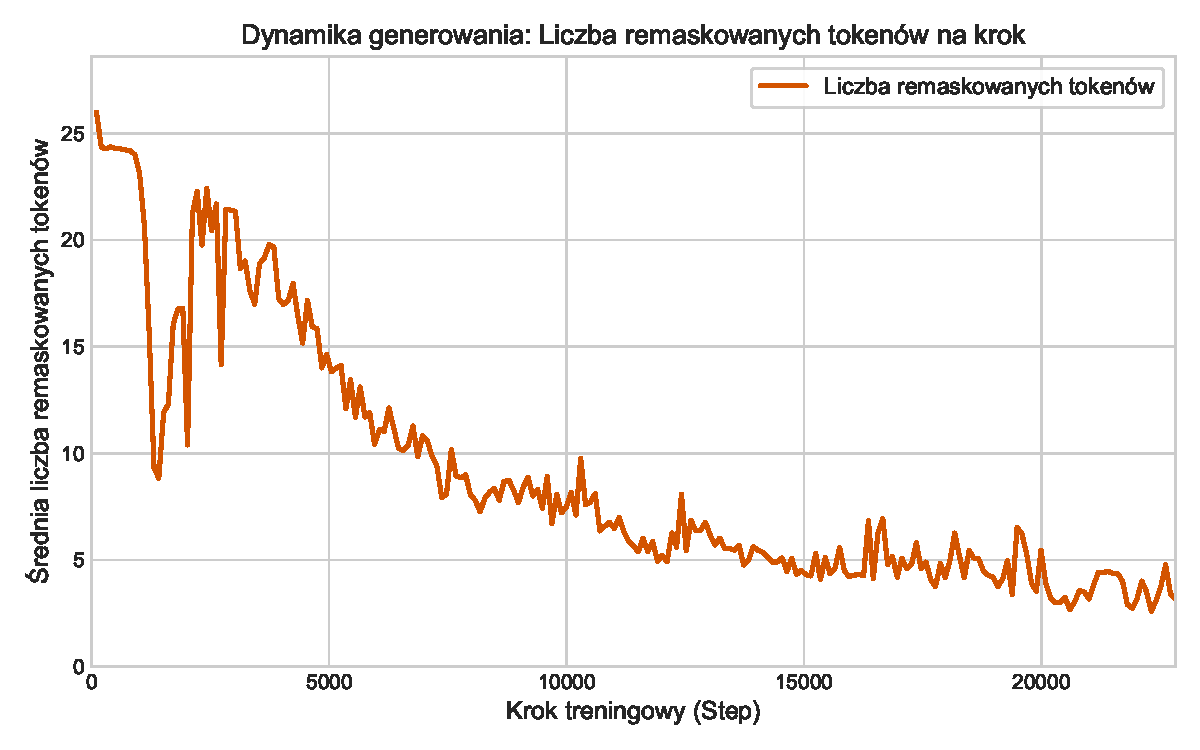
\includegraphics[width=0.85\linewidth]{figures/val_generation_remasking}
\caption{Średnia liczba tokenów oznaczanych jako niepewne i remaskowanych w pojedynczym kroku inferencji generatywnej w trakcie treningu.}
\label{fig:val-generation-remasking}
\end{figure}

Przedstawiony wykres ilustruje ewolucję dynamiki remaskowania w czasie. Na początku procesu treningowego model remaskuje średnio ok. \num{26} tokenów na krok, co świadczy o dużej niepewności w generowanych sekwencjach. W miarę postępu treningu średnia ta systematycznie spada, osiągając na końcu wartość ok. \num{2.6} tokena na krok. Spadek ten dowodzi, że model w kolejnych epokach generuje kod w sposób bardziej spójny i zdecydowany, produkując tokeny o wysokim prawdopodobieństwie już w pierwszych krokach generacji, co bezpośrednio skraca i stabilizuje iteracyjny proces próbkowania.
